\documentclass[11pt]{article}
\usepackage[margin=1in]{geometry}
\usepackage{amsmath,booktabs,graphicx,hyperref}
\title{Forecasting ETF Volatility and Returns\\{\large Model accuracy, the risk--return relationship, and portfolio outcomes}}
\author{IEDA 3330 project report}
\date{23 November 2026}
\begin{document}
\maketitle
\begin{abstract}
We forecast volatility and returns for three US equity ETFs. In the reserved 2026 volatility test, reducing the LSTM input sequence from 60 to 22 daily observations preserved five-trading-day forecast accuracy within the preset tolerance. Measured training time fell from 28.8 to 16.3 seconds in the earlier timing comparison. For the 22-trading-day forecast horizon, an LSTM correction improved on the statistical HAR baseline. Its advantage over a linear correction remained uncertain. In an exploratory analysis, we grouped forecast dates retrospectively by predicted risk. From the lowest to the highest monthly risk group, mean realized volatility rose from 4.46\% to 5.42\%, mean model-predicted return rose from 0.89\% to 1.14\%, and return forecast error rose from 4.18 to 6.02 percentage points. A portfolio holding fixed ETF allocations calibrated on earlier data earned more over the test period than daily HAR sizing at either horizon.
\end{abstract}
\begingroup
\hypersetup{hidelinks}
\setcounter{tocdepth}{2}
\tableofcontents
\endgroup
\clearpage
\section{Introduction}
At the market close, a risk manager may want to know both how widely an ETF's price could swing and whether taking that risk is likely to earn a higher return. A week of large price changes can end in either a gain or a loss. We first test how many daily observations a volatility model needs to process, then ask whether its risk estimates line up with independently forecast and subsequently realized returns. Finally, we measure the investment consequences of varying exposure with predicted risk.

French, Schwert and Stambaugh~\cite{french} study predictable market volatility and expected excess market returns. Here the unit of observation is an individual ETF on a forecast date, and the outcome is its total adjusted-price return. Pairing the two forecasts within each fund lets us ask whether relatively risky dates also carried higher predicted gains.
Figure~\ref{fig:experiment} traces the study from the pilot to the two follow-up analyses. The 2026 period was reserved for the volatility test. Both follow-ups reused those dates and are exploratory.

\begin{figure}[!ht]
\centering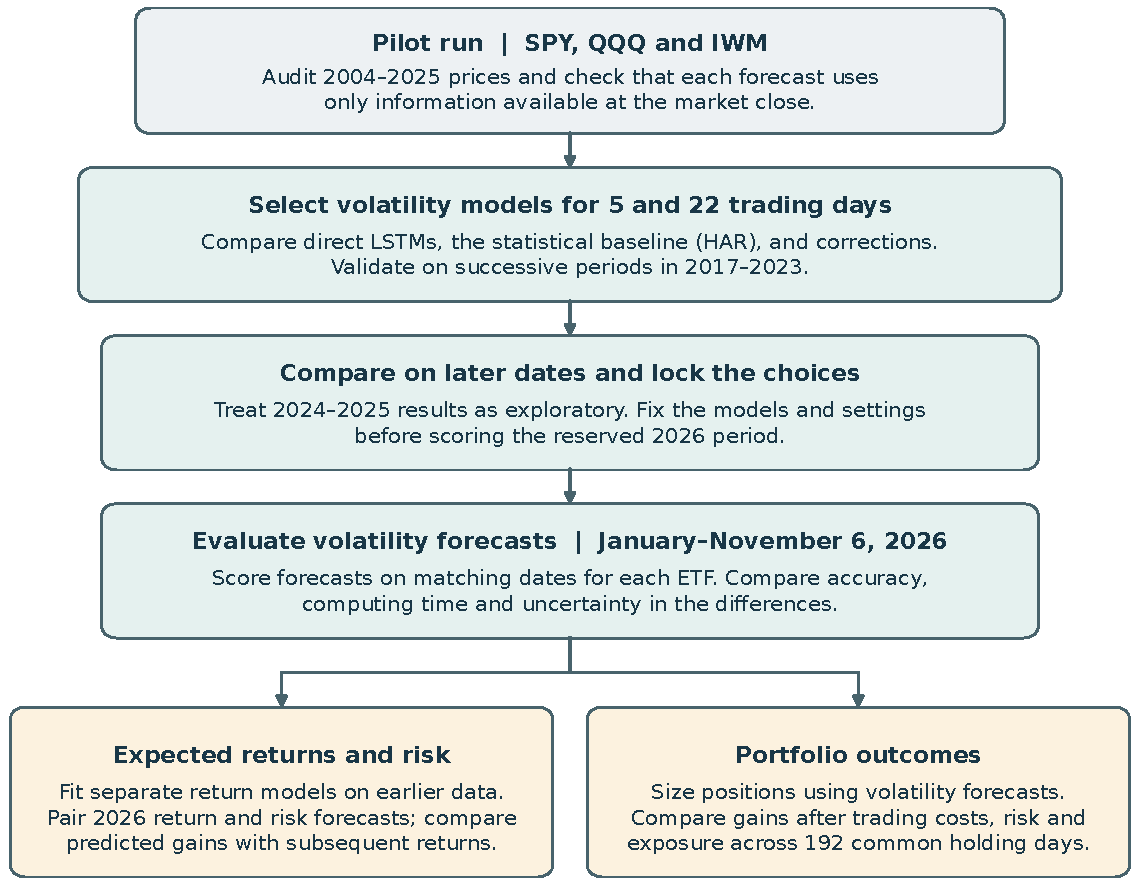
\includegraphics[width=.97\linewidth]{ETF_experiment_flowchart.pdf}
\caption{Experimental workflow. The return analysis pairs separately trained forecasts of risk and gain. The portfolio analysis uses the volatility forecast alone to decide how much to invest.}
\label{fig:experiment}
\end{figure}
\section{Data and design}
The pilot uses 5,535 Yahoo Finance daily records per ETF from January 2004 through December 2025. Session coverage, price consistency and corporate actions are audited. Let $r_t=\log(P_t/P_{t-1})$ for adjusted closes. A forecast issued after close $t$ targets $v_{t,h}=h^{-1}\sum_{j=1}^h r_{t+j}^2$, where $h=5$ or $22$. Annualized volatility is $\sqrt{252v}$. Inputs comprise return, absolute return, log trailing mean squared returns over 5, 22 and 60 sessions, log high/low, and log-one-plus volume centered on its 22-session mean.

\paragraph{Price snapshots.} The historical Yahoo Finance manifest records 7 November 2026 at 09:12 UTC. We used Yahoo's adjusted closing price for returns and the unadjusted high and low for the daily range. Both downloads requested corporate actions with automatic price adjustment and price repair disabled. The 2026 extension uses 31 December 2025 as an overlap date to align adjusted-close levels before appending the new sessions. Its separate manifest records checksums and session counts but omits the retrieval timestamp.

\paragraph{Why forecast five and 22 trading days ahead?} Five trading sessions cover about one week and 22 cover about one month. We chose these horizons before comparing model performance so we could ask whether a model that forecasts next week's volatility well also performs well over the coming month. Suppose we issue both forecasts for SPY on a Friday and its price moves sharply on Monday. Monday's squared return receives a weight of $1/5$ in the weekly average and $1/22$ in the monthly average. A single large move therefore matters more to the weekly measure. If large moves continue over the following weeks, the monthly measure captures them too. The horizon counts future sessions used to score the forecast. The lookback counts past sessions used to make it, so the same 60-session history can support either forecast.

For signed returns, the outcome is $R_{t,h}=P_{t+h}/P_t-1$. We match a return forecast and a variance forecast on fund, issue date, horizon and outcome date. To express forecast risk over those same days, we use $\sqrt{h\widehat v_{t,h}}$, an approximation to the standard deviation of cumulative log returns when daily means and serial covariances are small. Volatility errors and portfolio risk are reported on an annualized scale.

\paragraph{From volatility to portfolio risk.} Lecture 4 expresses portfolio variance as $w^\top\Sigma w$ and discusses the number of covariance estimates needed in practice. Our three forecasts approximate the diagonal of a daily covariance matrix under a small conditional-mean assumption: $E_t[r^2]=\operatorname{Var}_t(r)+(E_t[r])^2$. A portfolio of these ETFs also requires the three pairwise covariances. Equal weighting in our score tables averages forecast performance across funds; it does not estimate the volatility of an equal-weight portfolio.

Lecture 8 gives Gaussian value-at-risk as $\mu_L+\Phi^{-1}(\alpha)\sigma_L$ for loss $L$. For example, if the forecast average daily variance over five sessions were $0.0001$, then conditional Gaussian cumulative log loss with zero mean and uncorrelated daily innovations would have an approximate 95\% quantile of $1.645\sqrt{5(0.0001)}=3.68\%$ in log-loss units. The annualized volatility displayed in our charts would be $\sqrt{252(0.0001)}=15.87\%$. These two numbers answer different risk questions. The experiment scores the variance forecast; tail coverage would require a separate backtest.

\paragraph{Pilot.} We restarted training from the archived prices in a fresh run directory. The pilot used 2004 for warm-up, trained from 2005 and evaluated on 2024--2025. The GARCH(1,1) comparator updates conditional variance with the previous squared innovation and previous conditional variance~\cite{garch}. HAR instead combines daily, weekly and monthly averages, giving two distinct statistical benchmarks for the neural forecasts. The table reports equal-weight ETF means. MAE and RMSE use annualized volatility percentage points. Pilot results document pipeline operation.
\begin{table}[htbp]\centering\small\setlength{\tabcolsep}{4pt}\caption{Pilot accuracy on 2024--2025 data.}\label{tab:pilot}
\begin{tabular}{lrrrr}
\hline
Horizon & Pilot model & QLIKE & MAE & RMSE \\
\hline
5 & LSTM-ensemble & -7.961 & 6.144 & 9.398 \\
5 & HAR-style & -7.955 & 6.685 & 9.881 \\
5 & GARCH & -7.939 & 6.590 & 9.988 \\
22 & LSTM-ensemble & -7.806 & 5.559 & 8.607 \\
22 & HAR-style & -7.838 & 5.985 & 8.425 \\
22 & GARCH & -7.834 & 5.794 & 8.579 \\
\hline
\end{tabular}\end{table}
\section{Forecasting methods}
\subsection{Independent and dependent variables}
The \emph{independent variables}, or predictors, are market measurements available when the forecast is issued: recent returns, their size, measures of past volatility, the daily price range and relative trading volume. These measurements can be related to one another. The \emph{dependent variable} is the future outcome the model learns to predict. For volatility, it is the average squared daily return over the next five or 22 trading days. For expected return, the training outcome is the actual percentage gain or loss over those same days. A rise and a fall of similar size both increase the volatility measure, but they enter the return outcome with opposite signs.

\paragraph{One forecast from start to finish.} Suppose we issue a five-day SPY forecast after a Friday close. A short-window LSTM reads 22 trading days of indicators ending that Friday. The 22 days describe how far the model looks back; the five days describe how far ahead it predicts. After the next five sessions, their prices supply the two outcomes. During training, errors on completed historical examples guide changes to the network weights. During final evaluation, we score each issued forecast against its subsequent outcome. Those future prices were unavailable when the forecast was issued.

\paragraph{Why compare 22 and 60 past sessions?} About 22 trading sessions make up one month, and 60 cover roughly three months. We chose 60 as the reference and asked whether the most recent month of daily indicators would give comparable accuracy with less computation. For the same five-day SPY forecast, the longer window lets the model follow the sequence of daily changes before that last month. Each of its 22 rows contains indicators already calculated from earlier prices, including a trailing 60-session average of squared returns. Preparing those rows therefore requires more than 22 days of raw prices. We hold the fund, forecast horizon, scoring dates and network architecture fixed so that the comparison isolates the length of the input sequence.

For the five-day horizon, the 22-session window met the preset accuracy tolerance while processing 38 fewer daily inputs per forecast ($38/60 \approx 63\%$). For the 22-day horizon, validation retained the 60-session reference among the direct LSTMs. These findings apply to the two window lengths tested here. Tables~\ref{tab:volatility} and~\ref{tab:cost} give the forecast errors and measured computing times.

\subsection{Volatility models}
Lecture 9 introduces hidden layers as nonlinear transformations of predictors and illustrates a chronological train--validation--test split in a US equity application. Our recurrent implementation passes a learned state from one session to the next. This allows a feature such as a large absolute return to affect subsequent updates within a window, following the LSTM approach of Hochreiter and Schmidhuber~\cite{lstm}. A separate network is fitted for each ETF and horizon. Validation blocks are 2017--2018, 2019--2020 and 2021--2023. Training labels must mature before the validation block begins. The common training sample starts after 60 consecutive issued HAR forecasts from 2010. The reference uses 60 inputs in time, 32 hidden units and a 16-unit dense layer. Short uses 22 days, scalar additionally removes the dense layer, and narrow additionally reduces hidden width to 16. Each uses dropout 0.1 and a positive Softplus head. We average variance forecasts from seeds 17, 42 and 123. The Adam optimizer~\cite{adam} uses a learning rate of 0.001, batches of 32, gradient clipping at 1, a limit of 100 epochs and patience 10. Final fits use the median selected epoch across folds. Scalers use training rows alone.
\paragraph{Baseline and corrections.} Following the multiple-horizon construction of Corsi~\cite{corsi}, an expanding OLS regression uses daily, weekly and monthly squared-return averages. At each month end we update the coefficients using matured labels, effective next session. We floor the baseline $b$ at $10^{-8}$. Constant and regularized linear log multipliers serve as calibration controls. The hybrid reads the seven features and log issued baseline over 22 sessions with 16 hidden units. Its zero-initialized scalar head produces $z$, with $g=G\tanh(z/G)$ and $G=\log 4$. The forecast is $p=\max(10^{-8},b\exp g)$. We minimize $\log p+v/p+\lambda g^2$ and select $\lambda$ from 0, 0.01 and 0.1 (hybrid0, hybrid01 and hybrid1).
\begin{figure}[htbp]\centering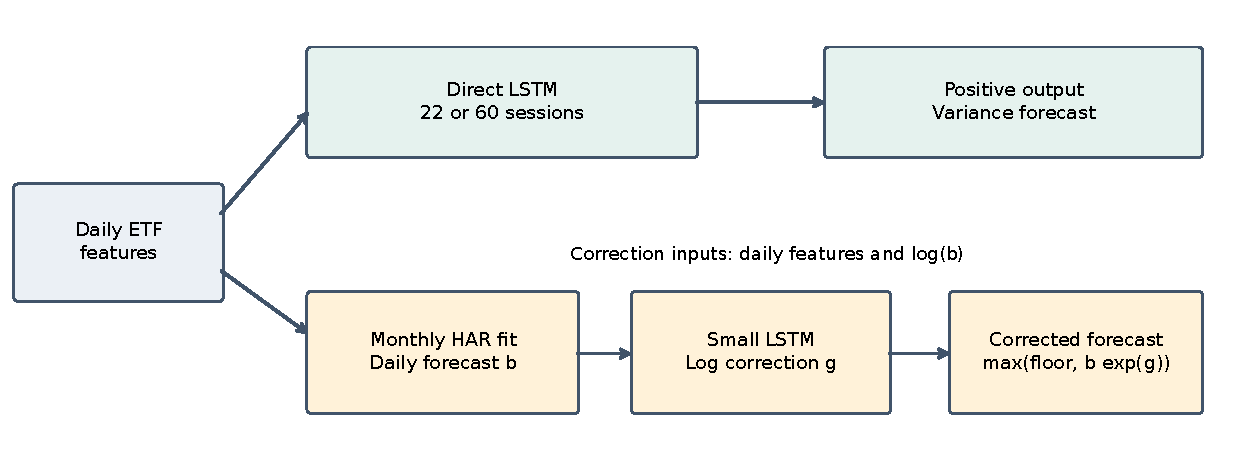
\includegraphics[width=\linewidth]{ETF_model_paths.pdf}
\caption{The direct network estimates variance from the feature window. In the correction model HAR issues the baseline first, then the small network estimates a log multiplier. A zero correction recovers the baseline.}\end{figure}
\paragraph{Selection and scoring.} Full QLIKE is $\log p+v/p$ and lower values indicate better performance. Patton~\cite{patton} analyzes forecast losses with imperfect volatility proxies. We select the fewest parameters within 0.005 of the best direct validation QLIKE, breaking ties using inference time. The hybrid minimizes validation QLIKE. Selection gives equal weight to folds and ETFs. The criterion retained the 22-session window with 32 hidden units and its dense layer for the five-day target. For the 22-day target it retained the 60-session reference. Both horizons selected a hybrid penalty of 0.1. The short model has the same number of weights as the reference but processes 63\% fewer recurrent steps. The 2024--2025 comparison is exploratory. January 1 through November 6, 2026 was reserved before selection. Only origins with all forward outcomes inside each evaluation period qualify. The 214 confirmation-period sessions per ETF are joined to the archived history by matching adjusted-close levels on December 31, 2025. Final confirmation weights use eligible training labels through 2025. The monthly HAR updates continue during evaluation.
\paragraph{What was fixed before scoring 2026.} The workflow specified the two primary comparisons, equal-weight mean QLIKE, paired date-block intervals and a tolerance of 0.005 QLIKE units. This was a researcher-chosen allowance for a small loss of accuracy in exchange for lower computing cost. The workflow gives no economic calibration for its size. The selection record saved on 18 November 2026 at 11:02 UTC identifies the chosen models, training durations and reserved dates before confirmation scoring. The period was a historical holdout. The return, risk-group and portfolio comparisons are exploratory.

\subsection{Return models and paired evaluation}
\paragraph{How we calculate expected return.} Let $P_t$ be the ETF's adjusted closing price on the forecast date and let $h$ be five or 22 trading days. Once those days have passed, the observed return is
\[
R_{t,h}=\frac{P_{t+h}-P_t}{P_t}.
\]
For example, a move from 100 to 102 gives an observed return of $2\%$. At the close on day $t$, the future price is still unknown. The model estimates the average return it expects given the information available at that close. We train and evaluate each fund and horizon separately.

\begin{description}
\item[Historical average.] Average all eligible $h$-day returns in the fund's training sample. This estimate stays fixed throughout the test period. A second baseline always forecasts zero.
\item[Linear model.] Start with the historical average and add a weighted adjustment for each of seven market indicators, including recent returns, trailing volatility and relative volume. The weights are learned from past outcomes, with a penalty on large coefficients.
\item[LSTM models.] The compact network reads 22 days of indicators using 16 hidden units. The reference network reads 60 days using 32 units and an intermediate layer. Both learn by minimizing squared differences between predicted and observed returns. For each configuration, we train three networks from different starting weights and average their forecasts. Validation on 2021--2023 sets the training duration; the final fits use eligible 2005--2025 examples.
\end{description}

\paragraph{A five-day SPY forecast.} At the January 2, 2026 close, the historical average predicted a gain of $0.23\%$, the linear model $0.18\%$, the compact LSTM $0.14\%$, and the reference LSTM $0.18\%$ (rounded). SPY subsequently gained $1.60\%$ through January 9. The January 2 estimates enter the forecast comparison; the January 9 price supplies the outcome used to calculate their errors. We report those errors in percentage points and measure skill by the reduction in squared error relative to the historical average.

\paragraph{From daily forecasts to the reported averages.} The reference LSTM's five-day mean forecast of $0.26\%$ in Table~\ref{tab:returns} averages 627 predictions: 209 forecast dates for each of three ETFs. For the monthly risk comparison in Table~\ref{tab:bands}, we first sort dates within each ETF by predicted volatility, then average the separately predicted 22-day returns in each group. This gives $0.89\%$ for the lowest-risk third and $1.14\%$ for the highest-risk third.

The 2026 period was reserved for the volatility test and subsequently reused for the return analysis. The latter is exploratory. Here predicted volatility changes roles: it is an output of the volatility model and then a grouping variable for comparing returns. A difference in gains across groups describes an association and cannot establish that volatility caused the difference. For each ETF, we group dates into thirds by hybrid HAR--LSTM risk, then compare average expected and realized returns. The cutoffs summarize the period retrospectively. We also rank dates within each ETF and measure the association between forecast risk and each return series. Uncertainty intervals resample consecutive dates jointly across funds, retaining dependence between overlapping outcomes.

\paragraph{Portfolio evaluation.} Following the idea of reducing exposure when volatility rises~\cite{moreira}, each ETF receives one third of the portfolio. The invested fraction of its sleeve is $\min(1,0.10/\sqrt{252\widehat v_{t,h}})$. For example, a 20\% annualized volatility forecast invests half of that ETF's allocation. Here predicted risk directly determines exposure, and subsequent ETF returns, exposure and trading costs together determine portfolio performance. A signal issued after today's close sets the position at the next close. Cash earns zero; trades cost 0.01\% of traded value. All policies face the same 192 close-to-close intervals from January 5 through October 9, 2026. Expected returns enter the paired forecast analysis; these portfolios use predicted volatility alone to size positions.

The 10\% setting applies to each ETF's one-third allocation. The volatility of the combined portfolio also depends on how the ETFs move together. This rule sizes positions from risk forecasts alone. It performs no mean--variance optimization.

\paragraph{Fixed-exposure comparison.} For each horizon and ETF, we applied the same sizing rule to the plain HAR forecasts issued in 2024--2025 and averaged the resulting portfolio weights over eligible dates (497 for five days and 480 for 22). We then held those target weights fixed and rebalanced daily in 2026, starting from cash and charging the same entry and rebalancing costs. In SPY, QQQ and IWM order, the five-day weights were 22.91\%, 17.88\% and 16.14\% of capital. The 22-day weights were 20.56\%, 16.79\% and 15.17\%. The balance stayed in cash. We designed this comparison after inspecting 2026 outcomes, using earlier data alone to set the weights. It compares daily timing with a similar typical allocation while allowing average exposure to differ in the test period.

\subsection{How to calculate QLIKE, MAE and RMSE}\label{sec:forecast-errors}
Start with one ETF, one model and one horizon (five or 22 trading days). For each of the $N$ forecast dates, record the predicted average daily variance $p_i$. Once the horizon ends, square each daily log return (written as a decimal) and average those squares to obtain the observed variance measure $v_i$.

\paragraph{QLIKE scores the variance forecast.} For each date, take the natural logarithm of the positive forecast and add the ratio of observed to predicted variance. Average these scores over the dates:
\[
\mathrm{QLIKE}=\frac{1}{N}\sum_{i=1}^{N}\left(\ln p_i+\frac{v_i}{p_i}\right).
\]
For example, suppose $v_i=0.0004$. A forecast of $0.0004$ scores $\ln(0.0004)+1=-6.824$. A forecast of $0.0001$ scores $\ln(0.0001)+4=-5.210$. The first forecast earns the lower (better) score. Negative scores are common because the logarithm of a small decimal variance is negative.

\paragraph{MAE and RMSE measure the size of a volatility miss.} First convert both variances to annualized volatility in percent, using 252 trading days per year. The error in percentage points is $e_i=100\sqrt{252p_i}-100\sqrt{252v_i}$. Mean absolute error (MAE) averages the sizes of the misses. Root mean squared error (RMSE) squares each miss, averages the squares and takes the square root:
\[
\mathrm{MAE}=\frac{1}{N}\sum_{i=1}^{N}|e_i|,
\qquad
\mathrm{RMSE}=\sqrt{\frac{1}{N}\sum_{i=1}^{N}e_i^2}.
\]
Suppose a model forecasts 18\% and 26\% annualized volatility on two dates and observed volatility is 20\% on both. The errors are $-2$ and $+6$ percentage points. MAE is $(2+6)/2=4.00$ points. RMSE is $\sqrt{(4+36)/2}=4.47$ points because squaring gives the larger miss more weight.

\paragraph{Reading the results tables.} In Table~\ref{tab:volatility}, we calculate each score separately for SPY, QQQ and IWM, then average the three fund scores equally. In Table~\ref{tab:returns}, RMSE uses the same formula with a different error: the predicted percentage gain or loss minus the observed percentage gain or loss over the full horizon. We pool those ETF-date errors and report RMSE in return percentage points without annualizing.

\section{Results}
\subsection{Forecast accuracy}
\begin{table}[htbp]\centering\small\setlength{\tabcolsep}{4pt}\caption{Volatility model selection on chronological validation periods.}\label{tab:validation}
\begin{tabular}{lrrr}
\hline
Horizon & Validation candidate & Parameters & QLIKE \\
\hline
5 & hybrid0 & 1681 & -8.0196 \\
5 & hybrid01 & 1681 & -8.0201 \\
5 & hybrid1 & 1681 & -8.0255 \\
5 & narrow & 1617 & -7.9475 \\
5 & reference & 5793 & -7.9852 \\
5 & scalar & 5281 & -7.9708 \\
5 & short & 5793 & -7.9843 \\
22 & hybrid0 & 1681 & -7.7070 \\
22 & hybrid01 & 1681 & -7.7077 \\
22 & hybrid1 & 1681 & -7.7196 \\
22 & narrow & 1617 & -7.6430 \\
22 & reference & 5793 & -7.7073 \\
22 & scalar & 5281 & -7.6827 \\
22 & short & 5793 & -7.6792 \\
\hline
\end{tabular}\par\vspace{6pt}\begin{minipage}{.97\linewidth}\small\setlength{\parskip}{4pt}
\textbf{Reading the columns.} The \emph{horizon} is the number of trading days ahead being forecast. A \emph{validation candidate} is a version tested on earlier periods to choose its settings. \emph{Parameters} counts the weights and biases learned by one network. QLIKE scores variance forecasts: lower is better, even when both scores are negative. Underestimating a large movement incurs a particularly large penalty.

\textbf{Reading the names.} The \texttt{reference} LSTM reads 60 days, keeps 32 internal memory values (hidden units), and uses a 16-unit intermediate layer to turn them into a forecast. \texttt{short} reads 22 days with the same network. \texttt{scalar} also removes the intermediate layer, and \texttt{narrow} further reduces the hidden units to 16. The three \texttt{hybrid} candidates start with HAR, a statistical volatility forecast, and learn an adjustment. The penalties for large adjustments are 0 (\texttt{hybrid0}), 0.01 (\texttt{hybrid01}) and 0.1 (\texttt{hybrid1}).

\textbf{Example.} For five-day forecasts, shortening the input window changed QLIKE from $-7.9852$ to $-7.9843$. The gap of 0.0009 was inside the preset tolerance of 0.005.
\end{minipage}\end{table}
Table~\ref{tab:volatility} compares models on the same forecast dates, giving equal weight to each ETF.
\begin{table}[htbp]\centering\small\setlength{\tabcolsep}{4pt}\caption{Volatility forecast accuracy on common dates. Errors are annualized volatility percentage points.}\label{tab:volatility}
\begin{tabular}{lrrrrrr}
\hline
Period & Horizon & Model & Origins & QLIKE & MAE & RMSE \\
\hline
explore & 5 & reference & 497 & -7.961 & 6.124 & 9.159 \\
explore & 5 & short & 497 & -7.953 & 6.263 & 9.299 \\
explore & 5 & HAR & 497 & -7.954 & 6.689 & 9.885 \\
explore & 5 & constant & 497 & -7.954 & 6.453 & 9.722 \\
explore & 5 & linear & 497 & -7.937 & 6.125 & 9.389 \\
explore & 5 & hybrid1 & 497 & -7.972 & 6.144 & 9.266 \\
explore & 22 & reference & 480 & -7.823 & 5.485 & 7.966 \\
explore & 22 & HAR & 480 & -7.836 & 5.987 & 8.436 \\
explore & 22 & constant & 480 & -7.837 & 5.835 & 8.337 \\
explore & 22 & linear & 480 & -7.797 & 5.678 & 9.338 \\
explore & 22 & hybrid1 & 480 & -7.838 & 5.449 & 8.102 \\
confirm & 5 & reference & 209 & -8.029 & 4.833 & 6.416 \\
confirm & 5 & short & 209 & -8.035 & 4.800 & 6.359 \\
confirm & 5 & HAR & 209 & -8.027 & 5.406 & 6.864 \\
confirm & 5 & constant & 209 & -8.029 & 5.231 & 6.718 \\
confirm & 5 & linear & 209 & -8.032 & 4.677 & 6.285 \\
confirm & 5 & hybrid1 & 209 & -8.050 & 4.691 & 6.280 \\
confirm & 22 & reference & 192 & -8.041 & 3.441 & 4.457 \\
confirm & 22 & HAR & 192 & -8.017 & 3.979 & 4.996 \\
confirm & 22 & constant & 192 & -8.028 & 3.807 & 4.781 \\
confirm & 22 & linear & 192 & -8.043 & 3.422 & 4.428 \\
confirm & 22 & hybrid1 & 192 & -8.045 & 3.369 & 4.341 \\
\hline
\end{tabular}\par\vspace{6pt}\begin{minipage}{.97\linewidth}\small\setlength{\parskip}{4pt}
\textbf{Reading the columns.} \texttt{explore} covers 2024--2025, already examined during development. \texttt{confirm} covers the reserved 2026 volatility evaluation. An \emph{origin} is a date on which a forecast was issued and its full outcome could later be scored. Counts are per ETF. QLIKE scores variance; MAE (mean absolute error) measures the average miss in annualized volatility percentage points. RMSE (root mean squared error) uses the same units and gives larger misses more weight. Lower is better for all three scores.

\textbf{Reading the baselines.} HAR combines daily, weekly and monthly averages of squared returns. \texttt{constant} multiplies HAR by one fitted factor throughout the evaluation period. \texttt{linear} lets that adjustment vary with market signals.

\textbf{Example.} For the 22-day confirmation forecasts, the average miss fell from 3.98 points with HAR to 3.42 with the linear correction and 3.37 with the LSTM correction. Most of the improvement over HAR was already available from the linear model.
\end{minipage}\end{table}
\paragraph{Cost.} Table~\ref{tab:cost} shows the computational savings from shortening the input window.
\begin{table}[htbp]\centering\small\setlength{\tabcolsep}{4pt}\caption{Measured CPU cost of the neural models.}\label{tab:cost}
\begin{tabular}{lrrrr}
\hline
Horizon & Network & Parameters & Train (s) & Inference ($\mu$s) \\
\hline
5 & reference & 5793 & 28.8 & 256.0 \\
5 & short & 5793 & 16.3 & 103.1 \\
5 & hybrid1 & 1681 & 11.1 & 54.4 \\
22 & reference & 5793 & 11.3 & 225.6 \\
22 & hybrid1 & 1681 & 5.5 & 50.4 \\
\hline
\end{tabular}\par\vspace{6pt}\begin{minipage}{.97\linewidth}\small\setlength{\parskip}{4pt}
\textbf{Reading the timings.} \emph{Network} identifies the model variant. \emph{Parameters} counts learned values in one network. \emph{Train (s)} measures fitting time in seconds. \emph{Inference} measures the time to produce a forecast after training, in microseconds ($\mu$s, one millionth of a second). Timings sum the three networks whose forecasts are averaged and are then averaged across ETFs. They exclude feature preparation and HAR refits and depend on CPU workload.

\textbf{Example.} The five-day \texttt{short} model took 16.3 seconds to train and 103 microseconds per forecast, compared with 28.8 seconds and 256 microseconds for \texttt{reference}. Both had 5,793 parameters: the shorter network ran faster because it applied the same weights over fewer days.
\end{minipage}\end{table}
\paragraph{Uncertainty.} Synchronized moving-block bootstrap intervals use 2,000 resamples of daily mean paired losses and block lengths of 20 or 66 sessions for five- or 22-day forecasts. A negative difference favors the candidate. The accompanying CSV includes sensitivity to shorter and longer blocks.
Adjacent 22-session targets share 21 daily returns. Following the block-resampling rationale for dependent observations~\cite{bootstrap}, we draw consecutive dates and keep all three ETFs together on each sampled date.

\textit{Exploratory period.} At five sessions the short-minus-reference loss difference was $+0.0074$; its interval crossed both zero and the preservation margin. The hybrid-minus-HAR intervals included zero at both horizons. These comparisons motivated caution in interpreting small score differences.

\textit{Reserved period.} The five-session short-minus-reference difference was $-0.0068$ with a 95\% interval of $[-0.0168,0.0037]$. Its upper endpoint fell below the prespecified $0.005$ margin, supporting preservation. A tighter allowance of $0.003$ would have changed that verdict. The five-session hybrid-minus-HAR interval crossed zero. At 22 sessions the hybrid-minus-HAR difference was $-0.0275$ with interval $[-0.0529,-0.0114]$. The direct selection at that horizon retained the reference, leaving no distinct simplified direct model to compare.

\paragraph{What accounts for the 22-session gain?} The hybrid reduced 2026 QLIKE relative to HAR for each ETF, by 0.047 for SPY, 0.010 for QQQ and 0.026 for IWM. A linear correction captured most of that gain. The hybrid-minus-linear difference was $-0.0022$ with an exploratory 95\% interval of $[-0.0084,0.0214]$. The data support correcting HAR, while the incremental value of the recurrent correction over linear calibration remains uncertain. The five-day preservation result and the 22-day hybrid-versus-HAR result held under all three reported block lengths.
\IfFileExists{ETF_LSTM_intervals.pdf}{\begin{figure}[ht]\centering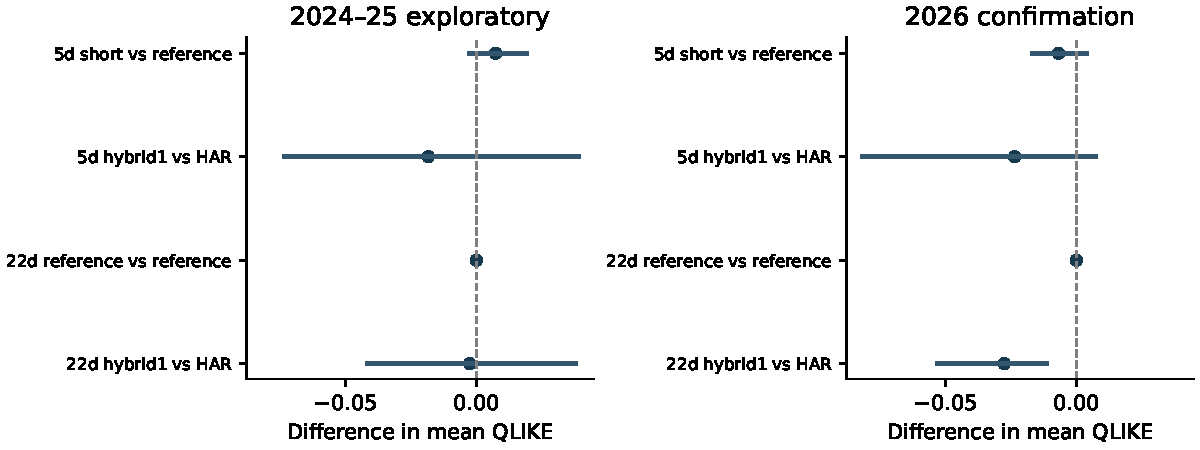
\includegraphics[width=\linewidth]{ETF_LSTM_intervals.pdf}\caption{Paired mean QLIKE differences and pointwise 95\% intervals. Negative values favor the candidate.}\end{figure}}{}
\begin{figure}[htbp]\centering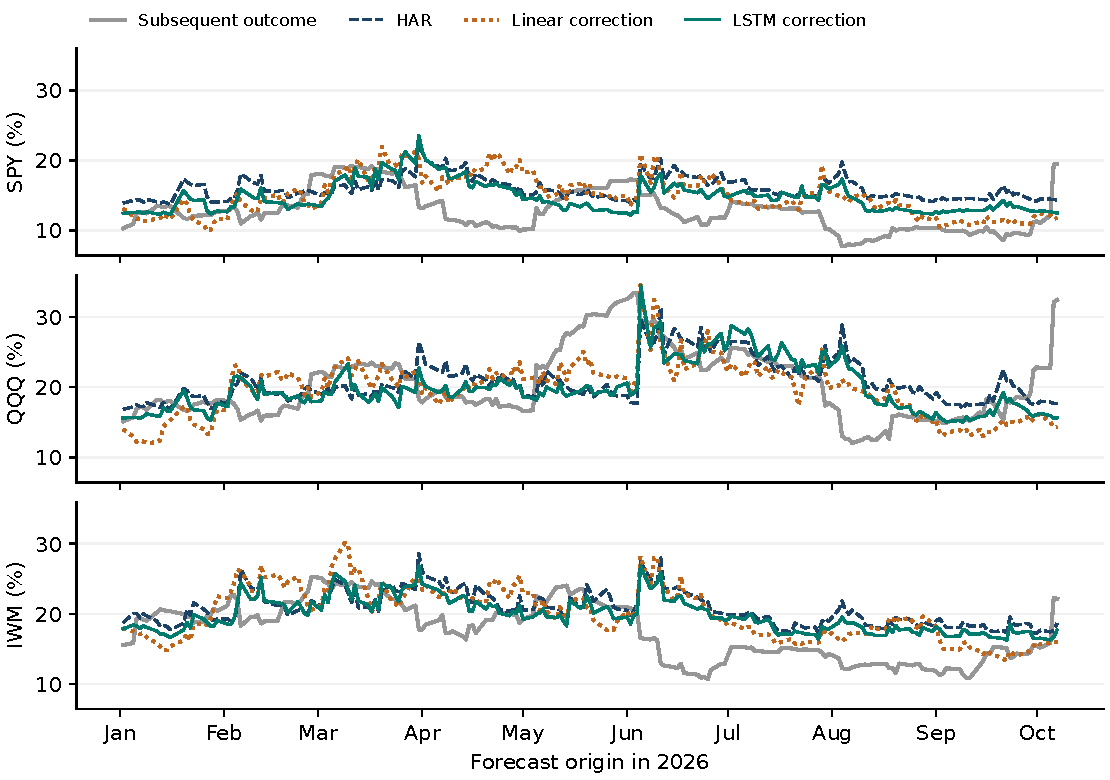
\includegraphics[width=\linewidth]{ETF_confirmation_paths.pdf}
\caption{Twenty-two-session forecasts for all three ETFs on the 192 common confirmation origins. Values are annualized volatility percentages. The gray outcome is aligned to the date the forecast was issued and becomes observable 22 trading sessions later. The two correction curves frequently overlap; the paired comparison in the text quantifies their difference.}\end{figure}

For returns, Table~\ref{tab:returns} compares the mean forecast, root mean squared error (RMSE, in percentage points) and skill against the historical average. The reference LSTM had the smallest RMSE at both horizons. Its reductions in squared error were 1.01\% and 1.74\%; both paired intervals included zero. Actual average gains were 0.24\% and 1.33\%. Evidence of improved return accuracy is weaker than the evidence for the monthly variance correction.

\begin{table}[htbp]\centering\small\setlength{\tabcolsep}{4pt}\caption{Accuracy of five- and 22-day return forecasts in 2026.}\label{tab:returns}
\begin{tabular}{lrrrrrr}\toprule
Return model & 5d forecast & 5d RMSE & 5d skill & 22d forecast & 22d RMSE & 22d skill \\ \midrule
Historical average & 0.25\% & 2.35 & 0.00\% & 1.11\% & 5.29 & 0.00\% \\
Zero return & 0.00\% & 2.36 & -1.03\% & 0.00\% & 5.46 & -6.48\% \\
Linear model & 0.24\% & 2.34 & 0.87\% & 1.09\% & 5.26 & 1.11\% \\
Compact LSTM & 0.22\% & 2.34 & 0.62\% & 0.71\% & 5.26 & 1.25\% \\
Reference LSTM & 0.26\% & 2.33 & 1.01\% & 1.01\% & 5.24 & 1.74\% \\\bottomrule\end{tabular}\par\vspace{6pt}\begin{minipage}{.97\linewidth}\small\setlength{\parskip}{4pt}
\textbf{Reading the columns.} 5d and 22d mean the next five and 22 trading days. \emph{Forecast} is the average predicted percentage gain or loss across dates and ETFs. \emph{RMSE} (root mean squared error) measures the size of the misses on individual forecasts, in percentage points, giving more weight to large errors. Lower is better. \emph{Skill} measures the percentage reduction in mean squared error against the historical-average model. Zero means a tie, and negative skill means larger errors.

\textbf{Reading the models.} Historical average always predicts the fund's average training-period return; zero return always predicts no change. The linear model adjusts the average using market indicators. The compact and reference LSTMs read sequences of 22 and 60 days, respectively. For the reference LSTM at 22 days, 1.01\% is the predicted average gain, 5.24 points is the RMSE, and 1.74\% is the reduction in squared error.
\end{minipage}\end{table}
\subsection{Do riskier dates carry higher expected returns?}
The matched sample contains 627 weekly and 576 monthly ETF-date observations. In the retrospective monthly groups, realized volatility rose from 4.46\% in the lowest predicted-risk third to 5.42\% in the highest. The reference LSTM predicted only 0.25 percentage points more return in the highest third. Its error was larger there as well (Table~\ref{tab:bands}). The observed gains in Figure~\ref{fig:bands} describe these dates in three related funds.

\begin{table}[htbp]\centering\small\setlength{\tabcolsep}{4pt}\caption{Volatility and returns by predicted-risk group. Both risk columns measure volatility over the forecast horizon.}\label{tab:bands}
\begin{tabular}{llrrrrr}\toprule
 & & \multicolumn{2}{c}{Horizon volatility} & \multicolumn{2}{c}{Return} & \\
Days & Risk group & Predicted & Realized & Predicted & Realized & RMSE (pts) \\ \midrule
5 & Low & 1.86\% & 1.99\% & 0.21\% & -0.09\% & 2.18 \\
5 & Middle & 2.29\% & 2.11\% & 0.23\% & 0.10\% & 2.30 \\
5 & High & 3.04\% & 2.80\% & 0.35\% & 0.71\% & 2.52 \\
22 & Low & 4.58\% & 4.46\% & 0.89\% & -0.90\% & 4.18 \\
22 & Middle & 5.22\% & 5.19\% & 1.01\% & 1.45\% & 5.35 \\
22 & High & 6.30\% & 5.42\% & 1.14\% & 3.43\% & 6.02 \\
\bottomrule\end{tabular}\par\vspace{6pt}\begin{minipage}{.97\linewidth}\small\setlength{\parskip}{4pt}
\textbf{Reading the groups.} We sorted dates within each ETF and horizon by predicted volatility and split them into thirds. For predicted volatility, multiply predicted daily variance by the horizon length and take the square root. Realized volatility is the square root of the sum of squared daily log returns over the same future days. We average those quantities within each group. The return columns average the reference LSTM's predicted gain and the subsequent signed gain.

\textbf{Reading the error.} For the high-risk 22-day group, the average predicted gain was 1.14\% and the average realized gain was 3.43\%. Their difference is 2.29 percentage points. The reported error of 6.02 points is larger because RMSE squares each individual miss before averaging; positive and negative misses cannot cancel.
\end{minipage}\end{table}
\begin{figure}[htbp]\centering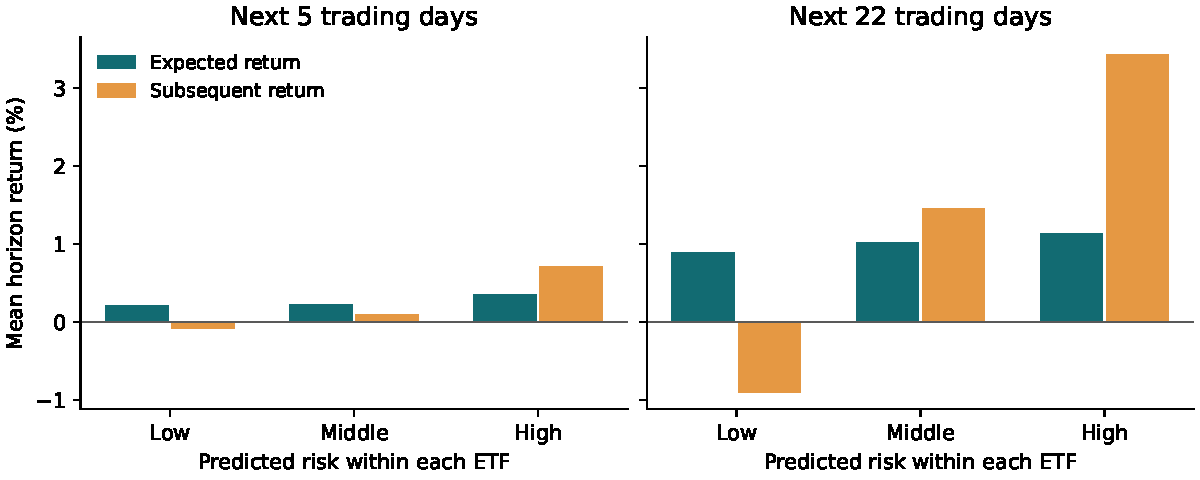
\includegraphics[width=.92\linewidth]{risk_bands.pdf}\caption{Mean expected and subsequent returns across forecast risk groups. Each panel covers one return horizon. The three groups are formed separately for each ETF.}\label{fig:bands}\end{figure}

Rank correlation measures whether riskier dates rank higher for returns (Table~\ref{tab:assoc}). The monthly association with realized returns was positive, while the weekly interval included zero. Using plain HAR risk kept the reference LSTM association positive (0.28 weekly and 0.70 monthly). Shared price inputs may explain some agreement between forecasts.
\begin{table}[htbp]\centering\small\setlength{\tabcolsep}{4pt}\caption{Mean within-fund rank correlations with hybrid risk. Brackets give pointwise 95\% intervals from 2,000 joint date-block resamples.}\label{tab:assoc}
\begin{tabular}{lrr}\toprule
Series compared with predicted risk & 5 days & 22 days \\ \midrule
Reference LSTM & 0.49 [0.27, 0.62] & 0.65 [0.43, 0.67] \\
Compact LSTM & 0.42 [0.25, 0.53] & 0.55 [0.32, 0.63] \\
Linear model & 0.22 [0.12, 0.29] & 0.13 [-0.03, 0.22] \\
Subsequent return & 0.15 [-0.07, 0.42] & 0.40 [0.16, 0.54] \\\bottomrule\end{tabular}\par\vspace{6pt}\begin{minipage}{.97\linewidth}\small\setlength{\parskip}{4pt}
\textbf{Reading the coefficients.} Each row compares two rankings of the same dates within each ETF. The first ranks dates by predicted volatility; the second ranks them by the named model's predicted return or, in the last row, by the return that actually followed. We average the three funds' rank correlations. A value near $+1$ means that higher-risk dates also tend to rank higher for returns; $-1$ means the order is reversed. Zero indicates no overall rank association.

\textbf{Reading the brackets.} The 95\% intervals show sampling uncertainty estimated by resampling runs of consecutive dates together across ETFs. At 22 days, 0.65 measures agreement between two forecasts. The last row's 0.40 compares predicted risk with actual returns. Its interval [0.16, 0.54] lies above zero; the five-day interval [$-0.07$, 0.42] leaves the direction uncertain.
\end{minipage}\end{table}
\subsection{Investment outcomes}
Table~\ref{tab:invest} reports net compounded gains, annualized mean daily returns, realized annualized risk and average capital invested. At five days, linear correction earned 8.20\% compared with 8.03\% for LSTM correction. At 22 days, the ordering reversed. The fully invested portfolio benefited more from the rising market and experienced nearly twice the volatility of several managed portfolios. Among the forecast-based strategies, none established a positive mean-return advantage over plain HAR in the paired intervals (Table~\ref{tab:portfolio-ci}).
\begin{table}[htbp]\centering\small\setlength{\tabcolsep}{4pt}\caption{Portfolio outcomes after assumed trading costs over the common holding period.}\label{tab:invest}
\begin{tabular}{lrrrrr}\toprule
Horizon & Sizing model & Net gain & Ann. mean & Ann. risk & Invested \\ \midrule
5d & Fixed exposure & 8.97\% & 11.68\% & 9.01\% & 56.93\% \\
5d & HAR & 7.11\% & 9.42\% & 8.90\% & 57.83\% \\
5d & HAR + constant & 7.31\% & 9.68\% & 9.15\% & 59.67\% \\
Both & Fully invested & 15.82\% & 20.58\% & 16.13\% & 100.00\% \\
5d & HAR + LSTM & 8.03\% & 10.57\% & 9.33\% & 62.92\% \\
5d & HAR + linear & 8.20\% & 10.81\% & 9.66\% & 64.80\% \\
5d & Reference LSTM & 7.61\% & 10.08\% & 9.47\% & 63.87\% \\
5d & Short LSTM & 7.83\% & 10.34\% & 9.41\% & 63.66\% \\
22d & Fixed exposure & 8.29\% & 10.80\% & 8.34\% & 52.52\% \\
22d & HAR & 7.20\% & 9.47\% & 8.33\% & 53.66\% \\
22d & HAR + constant & 7.31\% & 9.61\% & 8.46\% & 54.74\% \\
22d & HAR + LSTM & 7.60\% & 9.99\% & 8.71\% & 57.29\% \\
22d & HAR + linear & 6.85\% & 9.07\% & 8.68\% & 58.00\% \\
22d & Reference LSTM & 7.00\% & 9.25\% & 8.71\% & 57.72\% \\\bottomrule\end{tabular}\par\vspace{6pt}\begin{minipage}{.97\linewidth}\small\setlength{\parskip}{4pt}
\textbf{Reading the policies.} \emph{Horizon} identifies which volatility forecast sets the investment size each day. HAR uses the statistical baseline; constant, linear and LSTM corrections adjust that forecast daily. Fixed exposure keeps each ETF at its 2024--2025 average HAR weight. Reference and short LSTMs forecast volatility directly. \emph{Both} marks the fully invested benchmark, which uses the same daily equal-weight allocation for either horizon.

\textbf{Reading the outcomes.} \emph{Net gain} compounds daily portfolio returns over the 192 holding days after assumed trading costs. \emph{Ann. mean} puts the average daily net return on an annual scale by multiplying by 252. \emph{Ann. risk} measures realized volatility: the standard deviation of daily portfolio returns multiplied by $\sqrt{252}$. \emph{Invested} is the average share of capital held in ETFs; the balance is cash. For five-day HAR + linear, 8.20\% was earned over the test period, 10.81\% is the annualized arithmetic mean, and 64.80\% of capital was invested on average.
\end{minipage}\end{table}
\paragraph{Did varying exposure help?} Over the same 192 holding days, fixed weights earned 8.97\% against 7.11\% for weekly HAR sizing, and 8.29\% against 7.20\% for monthly HAR sizing. Fixed weights invested slightly less on average (56.93\% versus 57.83\% weekly and 52.52\% versus 53.66\% monthly), with similar realized risk. Plain HAR's annualized mean-return differences versus fixed weights were negative at both horizons, and both paired intervals lay below zero. The LSTM correction also earned less than fixed weights in this period, with intervals that included zero. A single exploratory period gives limited evidence about future timing performance.

\clearpage\begin{table}[!ht]\centering\small\caption{Annualized mean net-return differences in percentage points. Brackets give pointwise 95\% paired intervals.}\label{tab:portfolio-ci}
\begin{tabular}{llrr}\toprule
Days & Sizing model & Model minus plain HAR & Model minus fixed weights \\ \midrule
5 & Plain HAR & --- & -2.26 [-5.93, -0.22] \\
5 & HAR + constant & 0.27 [-0.25, 0.75] & -2.00 [-5.43, -0.17] \\
5 & HAR + linear & 1.39 [-3.62, 8.17] & -0.87 [-6.16, 4.05] \\
5 & HAR + LSTM & 1.16 [-2.93, 6.71] & -1.11 [-5.95, 3.52] \\
5 & Reference LSTM & 0.66 [-4.25, 7.42] & -1.60 [-7.00, 4.08] \\
5 & Short LSTM & 0.92 [-3.99, 7.83] & -1.34 [-6.72, 4.51] \\
22 & Plain HAR & --- & -1.33 [-3.52, -0.14] \\
22 & HAR + constant & 0.14 [-0.15, 0.41] & -1.18 [-3.26, -0.08] \\
22 & HAR + linear & -0.40 [-2.73, 1.50] & -1.72 [-4.20, -0.67] \\
22 & HAR + LSTM & 0.52 [-0.66, 1.61] & -0.81 [-2.79, 0.21] \\
22 & Reference LSTM & -0.21 [-2.05, 1.44] & -1.54 [-4.26, 0.03] \\
\bottomrule\end{tabular}\par\vspace{6pt}\begin{minipage}{.96\linewidth}\small
We compare net returns on the same holding days, multiply their mean difference by 252 and resample 20-day blocks 4,000 times. Positive values favor the named model. For monthly HAR + LSTM versus plain HAR, the estimate is $+0.52$ points and the interval spans $-0.66$ to $+1.61$. These intervals concern the annualized mean. Table~\ref{tab:invest} separately reports compounded gains over the test period.
\end{minipage}\end{table}

\section{Limitations and conclusion}
The five-day volatility model preserved forecast accuracy within the preset tolerance while processing a shorter sequence at lower measured cost. At the monthly horizon, correcting the HAR baseline improved variance forecasts, and a linear correction captured most of the gain. In the exploratory monthly comparison, the highest predicted-risk group had higher realized volatility, higher model-predicted gains and larger return forecast errors than the lowest group. Neither the return forecast comparisons nor the portfolio rankings establish a reliable expected-return advantage.

The three funds share US equity risk. Adjacent monthly outcomes share 21 trading days, so 192 dates supply substantially fewer independent observations. Intervals are pointwise, conditional on fitted models and sensitive to block length. The risk groups use cutoffs calculated after the period ended. To establish whether predicted volatility adds useful information about signed returns, a future study would need to compare otherwise identical return models with and without that input on fresh dates.
\section{Reproducing the comparisons}
The companion archive \texttt{ETF\_experiment\_code\_and\_data.zip} contains the price snapshots, training scripts, written workflow, selection record and saved forecasts. Its README gives commands for replaying the tables from forecasts and for refitting the models. The price manifests identify the snapshots by SHA-256 checksum. The file \texttt{forecast\_ledger.csv} records the ETF, issue date, outcome date, forecast variance and observed variance. \texttt{daily\_strategies.csv} records the signal, entry and exit dates, net return, turnover and exposure for every policy.

\paragraph{Chronological cutoffs.} Each training label becomes available at the close of the fifth or 22nd trading day after its forecast date. Its outcome must be known strictly before the evaluation block starts. During evaluation both issue and outcome must fall inside the block. The main volatility models use eligible training origins from 30 March 2010. The pilot and direct return models use eligible origins from 2005. The return models use the third validation block to select training duration and the final block for evaluation.

\begin{center}\small
\begin{tabular}{lrrr}\toprule
Stage & Last training outcome & First scored origin & Last scored outcome \\ \midrule
Validation 1 & 30 Dec 2016 & 3 Jan 2017 & 31 Dec 2018 \\
Validation 2 & 31 Dec 2018 & 2 Jan 2019 & 31 Dec 2020 \\
Validation 3 & 31 Dec 2020 & 4 Jan 2021 & 29 Dec 2023 \\
Exploratory & 29 Dec 2023 & 2 Jan 2024 & 31 Dec 2025 \\
Confirmation & 31 Dec 2025 & 2 Jan 2026 & 6 Nov 2026 \\
\bottomrule\end{tabular}\end{center}
For the final fit, the last training forecast dates were 23 December 2025 at five days and 28 November 2025 at 22 days. Both outcomes matured on 31 December. The last scored 2026 forecasts were issued on 30 October and 7 October respectively. Both matured on 6 November. The companion file \texttt{evaluation\_cutoffs.csv} gives the corresponding dates for every block and horizon.
\phantomsection
\addcontentsline{toc}{section}{References}
\begin{thebibliography}{10}
\bibitem{corsi} F. Corsi. A Simple Approximate Long-Memory Model of Realized Volatility. \emph{Journal of Financial Econometrics}, 7(2), 174--196, 2009. \href{https://doi.org/10.1093/jjfinec/nbp001}{Publisher record}.
\bibitem{patton} A. J. Patton. Volatility forecast comparison using imperfect volatility proxies. \emph{Journal of Econometrics}, 160(1), 246--256, 2011. \href{https://doi.org/10.1016/j.jeconom.2010.03.034}{Publisher record}.
\bibitem{lstm} S. Hochreiter and J. Schmidhuber. Long Short-Term Memory. \emph{Neural Computation}, 9, 1735--1780, 1997. \href{https://doi.org/10.1162/neco.1997.9.8.1735}{Publisher record}.
\bibitem{garch} T. Bollerslev. Generalized autoregressive conditional heteroskedasticity. \emph{Journal of Econometrics}, 31, 307--327, 1986. \href{https://doi.org/10.1016/0304-4076(86)90063-1}{Publisher record}.
\bibitem{adam} D. P. Kingma and J. Ba. Adam: A Method for Stochastic Optimization. ICLR, 2015. \href{https://arxiv.org/abs/1412.6980}{Author manuscript}.
\bibitem{bootstrap} H. R. K\"unsch. The Jackknife and the Bootstrap for General Stationary Observations. \emph{Annals of Statistics}, 17, no.~3, 1989. \href{https://doi.org/10.1214/aos/1176347265}{Publisher record}.
\bibitem{french} K. R. French, G. W. Schwert and R. F. Stambaugh. Expected stock returns and volatility. \emph{Journal of Financial Economics}, 19, 3--29, 1987. \href{https://doi.org/10.1016/0304-405X(87)90026-2}{Publisher record}.
\bibitem{moreira} A. Moreira and T. Muir. Volatility Managed Portfolios. NBER Working Paper 22208, 2016. \href{https://www.nber.org/papers/w22208}{Working paper}.
\end{thebibliography}
\end{document}
